%%%%%%%%%%%%%%%%%%%%%%%%%%%%%%%%%%%%%%%%%
% Beamer Presentation
% LaTeX Template
% Version 1.0 (10/11/12)
%
% This template has been downloaded from:
% http://www.LaTeXTemplates.com
%
% License:
% CC BY-NC-SA 3.0 (http://creativecommons.org/licenses/by-nc-sa/3.0/)
%
%%%%%%%%%%%%%%%%%%%%%%%%%%%%%%%%%%%%%%%%%

%----------------------------------------------------------------------------------------
%	PACKAGES AND THEMES
%----------------------------------------------------------------------------------------

\documentclass{beamer}

\mode<presentation> {

\usetheme{CambridgeUS}

}

\usepackage{graphicx} % Allows including images
\DeclareGraphicsExtensions{.png, .pdf}
\usepackage{booktabs} % Allows the use of \toprule, \midrule and \bottomrule in tables
\usepackage[parfill]{parskip}

%----------------------------------------------------------------------------------------
%	TITLE PAGE
%----------------------------------------------------------------------------------------

\title[Sublinear Space Pattern Matching]{The Theory and Practice of Sublinear Space Pattern Matching} % The short title appears at the bottom of every slide, the full title is only on the title page

\author{Dominic Moylett} % Your name
\institute[University of Bristol] % Your institution as it will appear on the bottom of every slide, may be shorthand to save space
{
University of Bristol \\ % Your institution for the title page
\medskip
\textit{dominic.moylett.2011@my.bristol.ac.uk} % Your email address
}
\date{\today} % Date, can be changed to a custom date

\begin{document}

\begin{frame}
\titlepage % Print the title page as the first slide
\end{frame}

%----------------------------------------------------------------------------------------
%	PRESENTATION SLIDES
%----------------------------------------------------------------------------------------

%------------------------------------------------
\section{Introduction}
%------------------------------------------------

\begin{frame}
\frametitle{Pattern matching}
Pattern matching refers to a collection of problems based fundamentally around the idea of `Where does this pattern occur in this text?'

This covers a wide variety of problems:
\begin{itemize}
    \item \textbf{$k$-mismatch:} Does this pattern occur with up to $k$ characters different?
    \item \textbf{Parameterised matching:} Does the text have similar structure to this pattern?
    \item \textbf{Dictionary matching:} Do any of these patterns occur in the text?
    \item \textbf{Regular Expressions:} \texttt{grep [a-zA-Z]+[0-9]*dm.}
\end{itemize}
\end{frame}

%------------------------------------------------

\begin{frame}
\frametitle{Sublinear space pattern matching}
It is easy to solve problems like the ones above in less space than it takes to store the text. This can be done by \textit{streaming} the text in one character at a time.

But can we solve these problems in less space than it takes to store the pattern?
\end{frame}

%------------------------------------------------
\section{The data is getting bigger}
%------------------------------------------------

\begin{frame}
\frametitle{`Big Data'}
``I remember when this topic was called `Massive Data'. Now it has gone from `Massive Data' to `Big Data'.''
\textit{Graham Cormode}\footnote{\url{https://youtu.be/AXsBQBzKfYw?t=35s}}
\end{frame}

%------------------------------------------------

\begin{frame}
\frametitle{What's the problem with big data?}
\begin{center}

\includegraphics[width=0.4\paperwidth]{moores_law}\footnote{\url{http://upload.wikimedia.org/wikipedia/commons/0/00/Transistor_Count_and_Moore\%27s_Law_-_2011.svg}}
\end{center}
``Sure, data's getting bigger, but so are our computers! Why can't we just throw more RAM at the problem?''
\end{frame}

%------------------------------------------------

\begin{frame}
\frametitle{May's Law}
``Software efficiency halves every 18 months, compensating for Moore's Law.''
\textit{David May}\footnote{\url{http://www.linux-mag.com/id/8422/}}
\end{frame}

%------------------------------------------------

\begin{frame}
\frametitle{Data is growing too fast}
Between 1999 and 2015, the size of RAM on commercial machines increased roughly 100 times over.\footnote{Calculated from \url{http://www.jcmit.com/memoryprice.htm}}

In comparison, between 1999 and 2012, the amount of webpages indexed at Google increased 1000 times over.\footnote{\url{http://readwrite.com/2012/02/29/interview_changing_engines_mid-flight_qa_with_goog}}
\end{frame}

%------------------------------------------------

\begin{frame}
\frametitle{More memory isn't always the answer}
Some devices we don't want to keep adding more RAM to.

We want to save physical space in routers and mobile phones to keep them small.

But at the same time, we want them to process a lot of data.

There has to be a compromise.
\end{frame}

%------------------------------------------------
\section{Why pattern matching?}
%------------------------------------------------

\begin{frame}
\frametitle{Broad applications}
Pattern matching is a generic collection of problems that have a wide range of applications:

\begin{itemize}
    \item Bioinformatics
    \item Web searching
    \item Plagiarism checking
\end{itemize}
\end{frame}

%------------------------------------------------

\begin{frame}
\frametitle{Space constraints}
Historically, pattern matching has required linear space. As the pattern grows, your data structure grows at the same rate.

However, Porat and Porat (2009) proved that with some chance of error, you can achieve pattern matching in logarithmic space, becoming the first to break this barrier.
\end{frame}

%------------------------------------------------

\begin{frame}
\frametitle{Other accomplishments}
Breslauer and Galil (2011) improved Porat and Porat's complexity from $O(n\log m)$ to $O(n)$ time.

Jalsenius, Porat and Sach (2012) created a solution to parameterised matching in sublinear space and $O(n)$ time.

Clifford et al. (to be published) created a solution to pattern matching with multiple patterns in sublinear space and $O(n\log m)$ time.
\end{frame}

%------------------------------------------------
\section{Looking ahead}
%------------------------------------------------

\begin{frame}
\frametitle{Some theory problems}
\begin{itemize}
    \item Parameterised matching
    \item Dictionary matching
    \item Parameterised dictionary matching
    \item Pattern matching against many texts
    \item $k$-mismatch
\end{itemize}
\end{frame}

%------------------------------------------------

\begin{frame}
\frametitle{Pattern matching under annotated streams}
Annotated data streaming is a recent model of computation proposed by Chakrabarti et al. (2012).

Alongside the data stream, the computer also has access to a second stream of extra information from a more powerful computer.

There are very few pattern matching solutions under this model right now.
\end{frame}

%------------------------------------------------

\begin{frame}
\frametitle{Pratical problems}
Very little research at practical performance of algorithms.

How can we make these algorithms run better in practice?

Can we incorporate practical concepts such as parallelism or vectorisation?
\end{frame}

%------------------------------------------------

\begin{frame}
\frametitle{Why are we suitable for this project?}
I developed the first implementation of Breslauer and Galil's algorithm for exact pattern matching, which yielded positive results:

\begin{center}
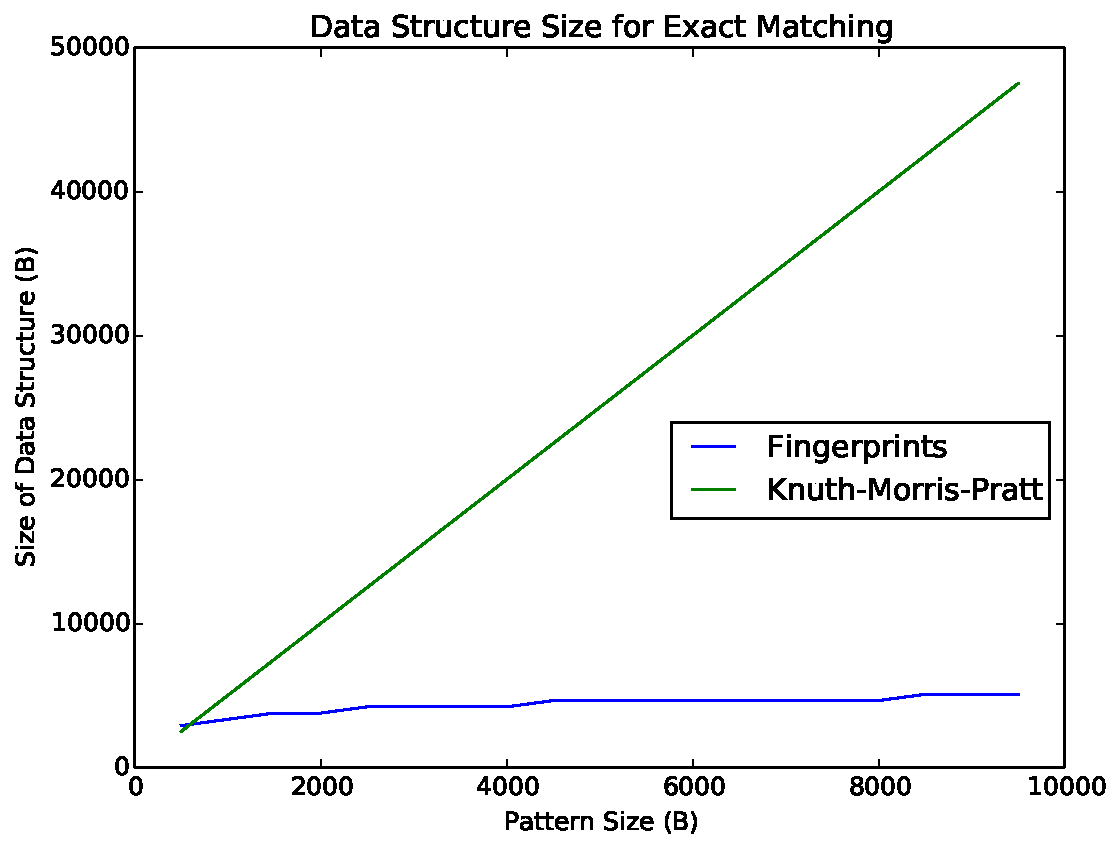
\includegraphics[width=0.5\paperwidth]{exact_size}
\end{center}

I have also spent this past six months working on the first implementation of Clifford et al.'s algorithm for dictionary matching.
\end{frame}

%------------------------------------------------

\begin{frame}
\frametitle{Work packages}
\begin{itemize}
\item\textbf{WP1:} (Years 1-2) Develop and improve algorithms for pattern matching problems in suiblinear space under the classic streaming model.
\item\textbf{WP2:} (Years 1-2) Develop new algorithms for pattern matching with annotated streams.
\item\textbf{WP3:} (Years 2-4) Implement new and recent algorithms to see how they perform when compared to classic methods on real data.
\end{itemize}
\end{frame}

%------------------------------------------------

\begin{frame}
\frametitle{Direction for Impact}
\begin{itemize}
\item\textbf{WP4:} (Years 4-5) Release implementations as tools for the open-source community.
\end{itemize}
\end{frame}

%------------------------------------------------
\section{The End}
%------------------------------------------------

\begin{frame}
\Huge{\centerline{Questions?}}
\end{frame}

%----------------------------------------------------------------------------------------

\end{document} 
